\documentclass[../main.tex]{subfiles}

\begin{document}

    \subsection{Aufbau des Lab 2, \glqq Würfel 1 bewegt sich und stösst\grqq{}}
    Für den Aufbau des Experimentes sind zwei Würfel mit den Dimensionen von 1.5m Seitenlänge und dem Gewicht von 2
    Kilogramm gegeben.
    Wie in der Abbildung~\ref{fig:2Lab_2dPictureNr1} zu entnehmen ist, wird der linke Würfel Julia und der rechte Romeo benannt.
    Daneben existiert eine Feder die horizontal an einer Wand befestigt ist.
    Bei dem gesamten Experiment wird der Reibungswiederstand ignoriert. \newline
    Ablauf des Experimentes:
 \begin{enumerate}
     \item Romeo wird mit einer konstanten Kraft (grüner Pfeil in Abbildung~\ref{fig:2Lab_2dPictureNr1}) auf
     2m/s nach rechts beschleunigt.
     \begin{figure}[H]
                 \begin{center}
                     \centerline{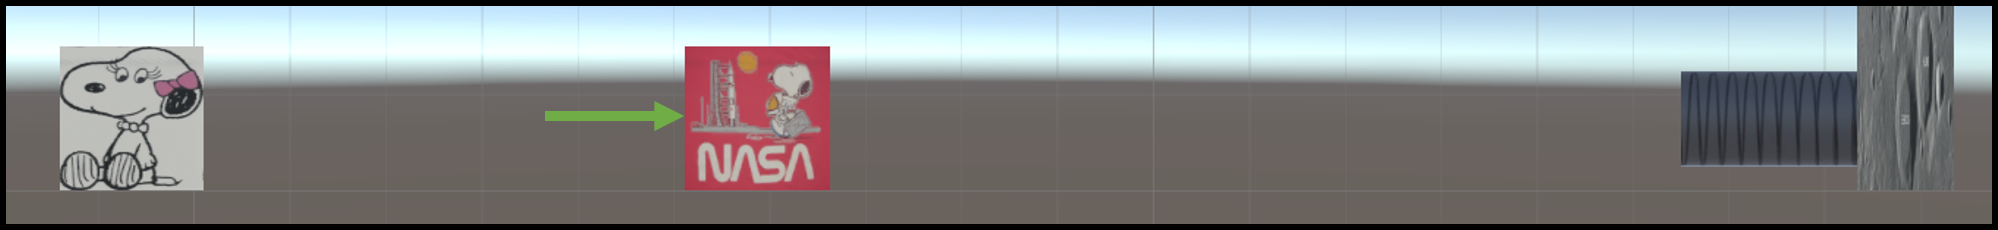
\includegraphics[width=155mm]{./images/2Lab_2dPictureNr1.png}}
                     \caption{Beschleunigung des Würfels}
                     \label{fig:2Lab_2dPictureNr1}
                 \end{center}
     \end{figure}
     \item Romeo trifft nun auf die Feder. Dabei soll die Federkonstante (gelber Pfeil in Abbildung~\ref{fig:2Lab_2dPictureNr2})
     so gewählt werden, dass Romeo elastisch zurückprallt ohne die Wand zu berühren.
     \begin{figure}[H]
               \begin{center}
                   \centerline{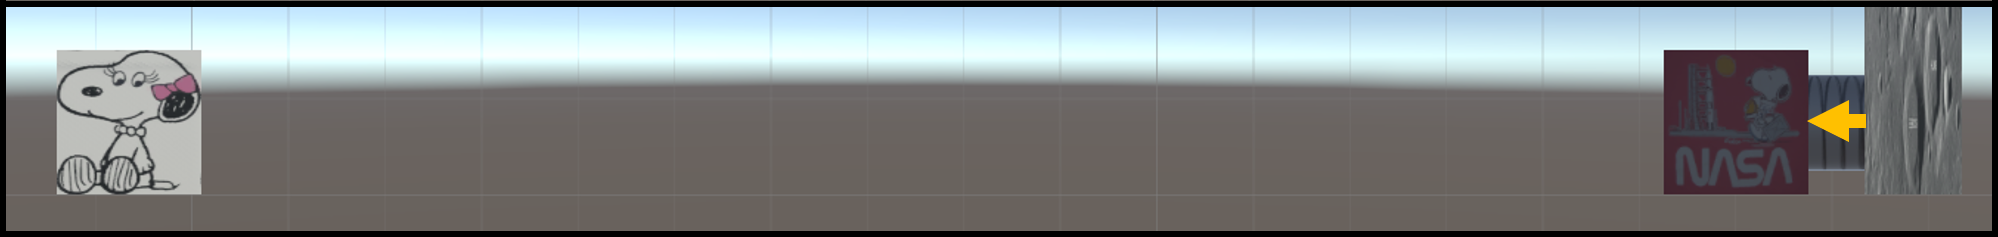
\includegraphics[width=155mm]{./images/2Lab_2dPictureNr2.png}}
                   \caption{Elastischer Zusammenstoss mit der Feder}
                   \label{fig:2Lab_2dPictureNr2}
               \end{center}
     \end{figure}
     \item Nach dem abgefederten Stoss gleitet Romeo zurück in die Richtung aus der er gekommen ist und stösst inelastisch mit Julia zusammen.
     Über einen FixedJoint haften die Beiden nun zusammen und gleiten mit der übertragener Energie
     (blaue Pfeile in Abbildung~\ref{fig:2Lab_2dPictureNr3}) weiter nacht links.
     \begin{figure}[H]
                \begin{center}
                    \centerline{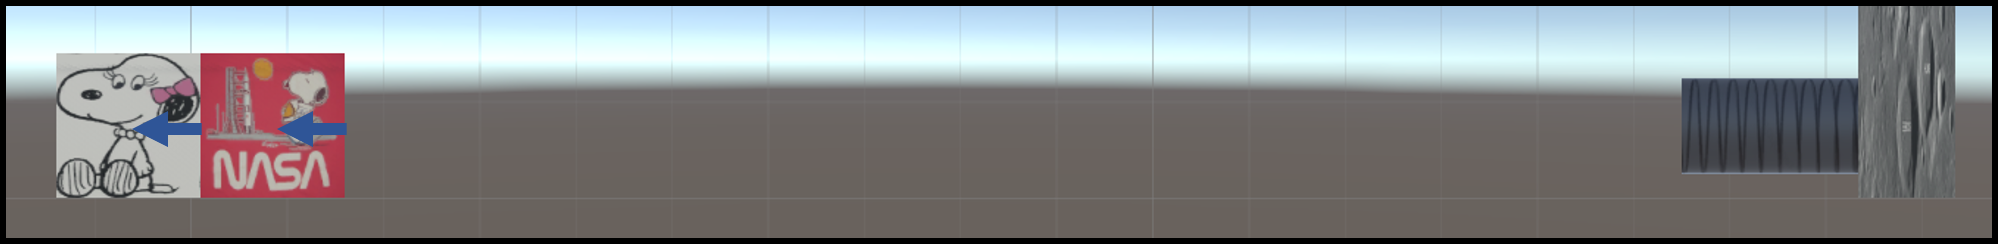
\includegraphics[width=155mm]{./images/2Lab_2dPictureNr3.png}}
                    \caption{Inelastischer zusammenstoss mit dem anderen Würfel}
                    \label{fig:2Lab_2dPictureNr3}
                \end{center}
     \end{figure}
 \end{enumerate}

    \subsection{Aufbau des Lab 3, \glqq Beide Würfel schwingen gedämpft\grqq{}}
    Nach dem zweiten Experiment gleiten die beiden Würfel noch einige Meter weiter,
    bevor sie von zwei Kranhaken an je einem 6 Meter langen Seil im Schwerpunkt aufgefangen werden.
    Dadurch schwingen Romeo und Julia hin und her. Während dieser Pendelbewegung verlieren sie
    kontinuierlich Impuls aufgrund des Luftwiderstands, bis sie schließlich zum Stillstand kommen.
    \newline
    Der gesamte Versuchsaufbau ist in Abbildung~\ref{fig:2Lab_2dPictureNr3} dargestellt.
    Es sollte jedoch beachtet werden, dass die Seile erst während des Experiments sichtbar
    werden. Diese sind pink markiert und in Abbildung~\ref{fig:3Lab_ExperimentOverview} zu sehen.
    \begin{figure}[H]
        \begin{center}
            \centerline{\includegraphics[width=155mm]{./images/3Lab_ExperimentOverview2d.png}}
            \caption{Schwingung des Würfels}
            \label{fig:3Lab_ExperimentOverview2d}
        \end{center}
    \end{figure}







\end{document}